\documentclass{llncs}
\usepackage{graphics}
\usepackage{amssymb}
\usepackage{amsmath}
\usepackage[dvips]{epsfig}
\usepackage[latin1]{inputenc}
\usepackage{url}

\def\CC{{C\hspace{-.05em}\raisebox{.4ex}{\tiny\bf ++}}~}
\addtolength{\textfloatsep}{-0.5cm}
\addtolength{\intextsep}{-0.5cm}


%%%%%%%%%%%%%%%% Titulo %%%%%%%%%%%%%%%
\title{Predicting Levels of Sales for Newly Published Books using Cost-Sensitive Ensemble Methods} 



%%%%%%%%%%%%%%%% autores %%%%%%%%%%%%%%
\author {}
\institute{}
% Antonio - Hossam add your 'official' e-mail here. ;)

\date{}

\begin{document}
\maketitle

%%%%%%%%%%%%%%%%%%%%%%%%%%%%%%%%%%%%%%%%%%%%%%%%%%%%%%%%%%%%%%
\begin{abstract}

\end{abstract}


%********************************************************************************

\section{Introduction}


\section{Materials and methods}
\subsection{Basic classifiers}


In order to show the need for more intelligent and complex classification models, basic and more common models are experimented and applied first. 
\begin{itemize}

\item \textbf{$k$-Nearest Neighbors ($k$-NN)}

\item \textbf{Naive Bayes classifier}

\item \textbf{C4.5 Decision Trees}


\item \textbf{Multilayer Perceptron neural networks (MLP)}: MLP is a feedforward 
artificial neural network model that maps the input data onto an appropriate output. 
It is an artificial neural network generally used for classification or 
approximation problems \cite{Rosenblatt1962,Widrow1990} .

This model is a generalisation of the standard linear perceptron that uses several 
layers of nodes (called neurons) and that is able to solve linearly inseparable 
problems \cite{SteinwenderBitzer2003}.
Each neuron consists of a linear combination of weighted inputs which is passed 
though a non-linear activation function to produce its output.

This kind of artificial neural network is trained using a supervised learning 
technique called back-propagation.
This training method was developed independently by Werbos \cite{Werbos1974}, 
Parker \cite{Parker1985} and Rumelhart et al. \cite{Rumelhart1985}, and consists
in updating the weights of the output layer neurons once the erroneous output 
has been obtained, and then, propagating the successive weight layers back to 
the input layer.

A key issue when designing an MLP is the number of hidden layers of neurons.
Lippmann proved in \cite{Lippmann1987} that two hidden layers are enough to 
create classifying regions of any kind. This result was then confirmed in later 
works by Bishop \cite{Bishop1996} and Reed et al. \cite{Reed1999}.

\item \textbf{Support Vector Machines (SVM)}


\end{itemize}






\subsection{Ensemble classifiers}

\begin{itemize}
\item \textbf{Bagging}
\item \textbf{Boosting}
\item \textbf{Random Forest}
\end{itemize}



\section{Cost sensitive classification}

\subsection{Cost sensitive learning}
\subsection{Cost sensitive classification}


\section{Dataset description}







The obtained dataset contains collected information about 6083 different books produced by 209 publishers. Each book in the dataset is represented by 10 feature as shown in Table \ref{tabla:params_pre_sales}. 


\begin{table}
\caption{Pre-sales features and Sales level(Output class). } 
\label{tabla:params_pre_sales}
\begin{center}
\begin{tabular}{|c|l|l|c|c|}
\hline 
No. & Feature Name & Variable & Type & In/Out\\
\hline 
1 & retail price (when launched) & \texttt{ret\_price} & numerical & input\\
2 & main subject (code) & \texttt{subject1} & numerical & input\\
3 & bookbinding (code) & \texttt{binding} & categorical & input\\
4 & gifts (promotional books) & \texttt{gifts} & numerical & input\\
5 & units distributed as novelty & \texttt{distrib\_novelty} & numerical & input\\
6 & total number of points of sale & \texttt{tot\_points\_sale} & numerical & input\\
7 & total number of points of sale (1st year) & \texttt{tot\_points\_sale\_1st\_year} & numerical & input\\
8 & weeks on sale & \texttt{weeks\_sale} & numerical & input\\
9 & print run & \texttt{print\_run} & numerical & input\\
\hline 
\hline
10 & Sales level & \texttt{sales\_level} & categorical & output\\
\hline 
\end{tabular}
\end{center}
\end{table}


The output variable which is the total sales is a categorical variable the represent the level of the quantity sold of a given book. Four categories are used to represent the total sales level: Low (L), Medium (M), High (H) and Very High (VH). Table \ref{table:freq} shows the ranges of total sales that correspond to each category along with the number of sold books that fall in. 

Table \ref{table:freq} and Figure \ref{fig:count} reveal more information about the nature of the dataset. We can notice that most of 77\% of the boos investigated are categorized as VL and L with limited number of sales. On the other side, the books that achieved more than 2000 sold copies are just around 4\%. This makes the problem of identifying those two categories much harder. The new categorical feature is used to replace the old numerical Total Sales feature in the GP classification case.

\begin{table*}[ht]
\caption{Categories corresponding to total sales }
\centering{}%
\begin{tabular}{|c|c|c|c|}
\hline 
Category & Range of total sales & Count & Ratio\tabularnewline
\hline 
\hline 
Low & 0-60 & 1631 & 26.8\%\tabularnewline
\hline 
Medium & 61-300 & 2212 & 36.4\%\tabularnewline
\hline 
High & 300-1000 & 1460 & 24\%\tabularnewline
\hline 
Very High & $>$1000 & 780 & 12.8\%\tabularnewline
\hline 
\end{tabular}
\label{table:freq}
\end{table*}



\section{Evaluation measurements}

To evaluate the developed classification models, first, we refer the confusion matrix shown in Table \ref{fig:confusionmatrix} which is considered as a basic source for evaluating any binary classification model. In our case which is a multiclass prediction problem, this matrix can be expanded with a row and column for each class to evaluate the multiclass classfication models. Three measurements are used to evaluate the applied classifiers: accuracy rate, precision and recall. The accuracy rate simply measures the total number of correctly classified instances over the total number of instances $N$ as shown in Equation \ref{equation:acc}.

Precision is the ratio of the correctly classified instances as $i$ to the number of instances classified as $i$. On the other side, recall is the ratio of the correctly classified instances as $i$ to the number of actual $i$ instances . Precision and recall are given in Equation \ref{equation:precision} and \ref{equation:recall}, respectively.


\begin{figure*}[ht]
\begin{center}
\includegraphics[scale=0.50]{confusion-matrix}
\end{center}
\caption{Basic confusion matrix.}
\label{fig:confusionmatrix}
\end{figure*}

\begin{equation}
Accuracy=\frac{\sum_{i}C_{ii}}{N}
\label{equation:acc}
\end{equation}


\begin{equation}
Precision_{i}=\frac{C_{ii}}{\sum_{j}C_{ij}}
\label{equation:precision}
\end{equation}


\begin{equation}
Recall_{i}=\frac{C_{ii}}{\sum_{j}C_{ji}}
\label{equation:recall}
\end{equation}

\begin{figure*}[ht]
\begin{center}
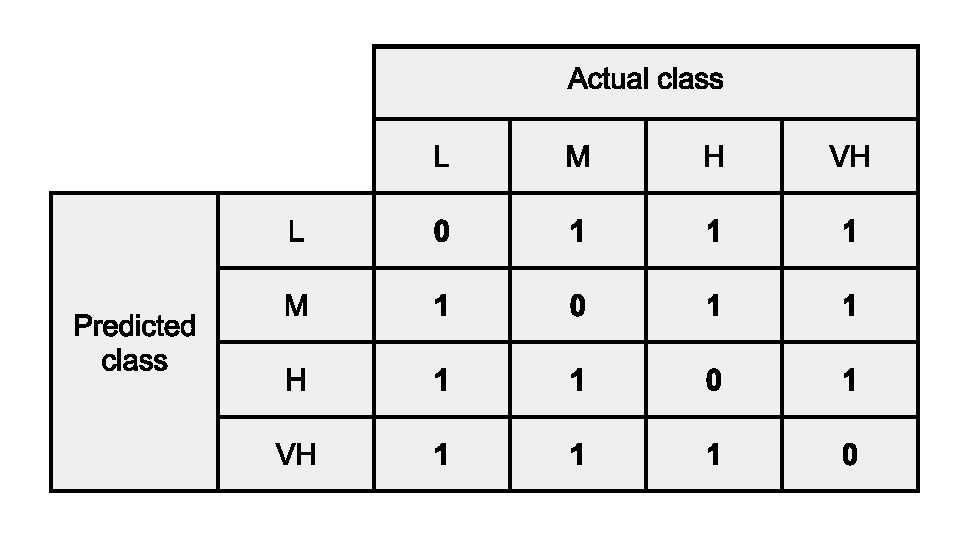
\includegraphics[scale=0.40]{Confusion-matrix-multiclass-default}
\end{center}
\caption{Default cost matrix.}
\label{fig:count}
\end{figure*}





\section{Experiments and results}

%This is just the first step of the experiments
% This table shows the average results of 10X10-folds experiments of the basic classifiers.
% It is impossible to calculate directly the average Precision and Recall for each class for multiclass problems in Weka Experimenter. So I have written a bash script to generate the row predictions utilizing Weka 3.9 developers version. Then I wrote another Python script to process these predicitons and calculate the precision and recall measurements as listed in this table.



\begin{table}
\caption{Classification results using basic classifiers}
\begin{centering}
\begin{tabular}{|c|c|c|c|c|c|}
\hline 
 & kNN & NB & J48 & MLP & SVM\tabularnewline
\hline 
\hline 
$Accuracy$  & 0.69$\pm$0.0018 & 0.66$\pm$0.001 & 0.7$\pm$0.0029 & 0.71$\pm$0.0022 & 0.67$\pm$0.0011\tabularnewline
\hline 
\hline 
$Recall_{L}$ & 0.76$\pm$0.0035 & 0.87$\pm$0.0013 & 0.79$\pm$0.0073 & 0.78$\pm$0.0178 & 0.6$\pm$0.0023\tabularnewline
\hline 
$Precision_{L}$ & 0.78$\pm$0.0027 & 0.71$\pm$0.0009 & 0.79$\pm$0.006 & 0.81$\pm$0.0166 & 0.84$\pm$0.0018\tabularnewline
\hline 
\hline 
$Recall_{M}$ & 0.74$\pm$0.003 & 0.64$\pm$0.0018 & 0.69$\pm$0.0074 & 0.71$\pm$0.0205 & 0.82$\pm$0.0015\tabularnewline
\hline 
$Precision_{M}$ & 0.65$\pm$0.0019 & 0.63$\pm$0.0009 & 0.68$\pm$0.0051 & 0.68$\pm$0.0084 & 0.6$\pm$0.0009\tabularnewline
\hline 
\hline 
$Recall_{H}$ & 0.59$\pm$0.0019 & 0.53$\pm$0.0018 & 0.6$\pm$0.0118 & 0.65$\pm$0.0399 & 0.56$\pm$0.0024\tabularnewline
\hline 
$Precision_{H}$ & 0.62$\pm$0.0021 & 0.58$\pm$0.0022 & 0.61$\pm$0.0061 & 0.62$\pm$0.0109 & 0.63$\pm$0.0016\tabularnewline
\hline 
\hline 
$Recall_{VH}$ & 0.61$\pm$0.005 & 0.52$\pm$0.0046 & 0.72$\pm$0.011 & 0.67$\pm$0.0277 & 0.61$\pm$0.0021\tabularnewline
\hline 
$Precision_{VH}$ & 0.78$\pm$0.0063 & 0.82$\pm$0.0028 & 0.73$\pm$0.0076 & 0.77$\pm$0.0213 & 0.78$\pm$0.0027\tabularnewline
\hline 
\end{tabular}
\par\end{centering}

\end{table}

%********************************************************************************
\section{Conclusions and Future Work}
\label{sec:conclusionsAndFutureWork}





%********************************************************************************
\section*{Acknowledgements}



%********************************************************************************
\bibliographystyle{plain}
\bibliography{refs}

%----------------------------------------------------------------------

\end{document}
%%% Local Variables:
%%% ispell-local-dictionary: "english"
%%% End:
